\documentclass[twocolumn,superscriptaddress,aps]{revtex4-1}

\usepackage[utf8]{inputenc}

\usepackage{amsfonts}
\usepackage{amssymb}
\usepackage{amsmath}
\usepackage{amsthm}

\usepackage{bbold}
\usepackage{bm}
\usepackage{color}
\usepackage{hyperref}
\usepackage{graphicx}
\graphicspath{{figures/}}

\begin{document}


% ==============================================================================

\title{\Large{INFO8010: Brain Cancer Detection Project Report}}
\vspace{1cm}
\author{\small{\bf Ayoub Assaoud}}
\affiliation{\texttt{ayoub.assaoud@student.uliege.be} (\texttt{s207227})}

\maketitle
\section{Abstract}

\section{Introduction}
%%% Introduction: which states the problem which has been tackled

For this project we propose to build a generative deep learning system that can generate anime faces. The system will be trained on a dataset of anime faces and will use denoising diffusion probabilistic models (DDPM) to generate new faces. The goal is to create a system that can generate acceptable quality anime faces that are diverse and realistic by drawing samples, and naturally for denoising by encoding-decoding the image. The project will also explore the use of different architectures and techniques to improve the quality of the generated faces.

Through this project, we:

\begin{itemize}
        \item Collecte and preprocess over than 80,000 anime face images, applying normalization, resizing, and few augmentations.
        \item Design and train two distinct deep learning models, mainly noise prediction technique and have a quick view on score-based energy model, experimenting with different architectures and training strategies.
        \item Evaluate performance using some basic metrics.
\end{itemize}
In the following sections, we'll walk through related work, our data pipeline, model Architecture, and results.

\section{Related Work}
%%% Related Work: which covers research that is related to the considered problem
\subsection{Denoising Diffusion Probabilistic Models}

Denoising Diffusion Probabilistic Models (DDPM), introduced by Ho et al.~\cite{ho2020ddpm}, laid the foundation for a class of generative models that iteratively reverse a diffusion process to synthesize high-quality data samples. The original DDPM framework employs a convolutional U-Net architecture to model the denoising function, demonstrating impressive results in image generation without relying on attention mechanisms. Subsequent works have extended this paradigm by integrating transformers to better capture long-range dependencies and enable multimodal conditioning, particularly in text-to-image synthesis tasks. Models such as GLIDE~\cite{nichol2021glide}, Imagen~\cite{saharia2022imagen}, and DALL·E 2~\cite{ramesh2022hierarchical} exemplify this shift, incorporating transformer-based components to enhance expressiveness and scalability.

Our work builds on this trajectory by exploring the role of transformers within the DDPM framework, aiming to enhance diffusion modeling with the representational power of attention-based architectures, as well as the limitations.

\subsection{Modified Forward Diffusion Kernel}
Recent efforts have explored modifications to the forward diffusion kernel in DDPMs to improve sampling efficiency and image quality. The LearnOpenCV guide~\cite{learnopencv2023ddpm} discusses a variant where the noise schedule and kernel are adapted to better preserve semantic structure during the forward process. By refining the way noise is injected, this approach aims to maintain more meaningful latent representations, which in turn facilitates more accurate denoising during reverse diffusion. Such kernel-based modifications offer a promising direction for enhancing DDPMs without fundamentally altering their probabilistic framework. Our work complements these ideas by investigating how transformer-based architectures can further improve the expressiveness and flexibility of the denoising model, especially when combined with advanced kernel designs.

\href{https://learnopencv.com/denoising-diffusion-probabilistic-models/#modified-forward-diffusion-kernel}{Modified Forward Diffusion Kernel}

\section{Methods}
%%% Methods: a clear and detailed description of the neural networks (architecture, training-parameters, loss function, data)
\subsection{Data}
\subsubsection{Dataset Description}

we took the \href{https://www.kaggle.com/datasets/splcher/animefacedataset/}{\textbf{Anime Face Dataset}} ($63k$ images), in addition to \href{https://www.kaggle.com/datasets/soumikrakshit/anime-faces}{\textbf{soumikrakshit Anime Face}} ($21k$ images).
%TODO: some image samples
% \begin{figure}[htbp]
%     \centering
%     \includegraphics[width=0.5\textwidth]{figures/dataset_sample.png}
%     \caption{A sample of MRI images from the brain tumor dataset.}
%     \label{Figure 1: dataset}
% \end{figure}

\subsubsection{Data Preprocessing}
Our preprocessing pipeline was implemented in Python using PyTorch library, and included the following steps:

\begin{itemize}
    \item \textbf{Cleaning}: To insure the quality of dataset, we removed all images for which the size is less than 64x64, resulting in 80k remaining images.
    \item \textbf{Resizing:} All images were resized to a fixed size of 64x64 pixels.
    \item \textbf{Normalization:} We normalize the pixel values to the range [-1, 1], to keep consistent with the noise distribution. an it seems to be much more effective than constraining the model to output values in the [0, 255] range, as it allows for better training stability and convergence.
    \item \textbf{Data Augmentation:} We applied random horizontal flipping to increase dataset diversity, no rotation or cropping was applied because most faces were not centered, or touching the frame, which could lead to poor generated samples.
\end{itemize}

%%%%%%%%%%%%%%%%%%%%%%%%%%%%%%%%%%%%%%%%%%%%%%%%%%%%%%%%%%%%%%%%%%%%%%%%%%%%%%%%%%%%%%%
\subsection{Architecture}
We use a denoising diffusion probabilistic model (DDPM) as the backbone of our generative system. The DDPM consists of a forward diffusion process that gradually adds gaussian noise to the data, and a reverse diffusion process that learns to denoise the data. This architecture allows for high-quality image generation by sampling from the learned distribution.

the same architecture can be used to approximate the score function of the data distribution $s_\theta(x , t) \approx \nabla \log p_t(x_t)$.

\subsubsection{Description}

We explore several variants of the DDPM architecture, including:

\begin{itemize}
    \item \textbf{U-Net:} A U-Net architecture is used as the denoiser model that predicts the original noise $\epsilon \approx\epsilon_\theta(x_t, t)$ for the DDPM.
    \item \textbf{ResNet Blocks:} We incorporate residual blocks to improve the flow of gradients during training, which helps in learning complex features.
    \item \textbf{Attention Mechanisms:} We incorporate attention mechanisms to improve the model's ability to focus on relevant features during the denoising process.
\end{itemize}

The Unet architecture consists of Three main components: a chain of $down_channels$ \textbf{DownEncoder}, a chain of $mid_channels$ \textbf{Bottleneck}, and a chain of $down_channels$ \textbf{UpDecoder}, to preserve symmetric feature mapping.

The DownEncoder reduces the spatial dimensions of the input image while increasing the number of feature channels, allowing the model to learn hierarchical representations.

The Bottleneck connects the DownEncoder and UpDecoder, serving as a bridge that captures the most abstract features.

The UpDecoder then reconstructs the image by progressively increasing the spatial dimensions while reducing the number of feature channels (Up sampling) and concatenates the correspondding levels DownEncoder outputs with those of the UpDecoder.

Each of these subcomponents is composed of \small{$ModelParams.num\_(down\|mid\|up)\_layers$} \textbf{block layers}, each of these block layers consists of a stack of ResNet block followed by a self-attention layer (optionnel in our case see discussion) and finally an optionnel convolutive layer (downsampling or upsampling), see figure bellow.

\begin{figure*}[ht]
  \centering
  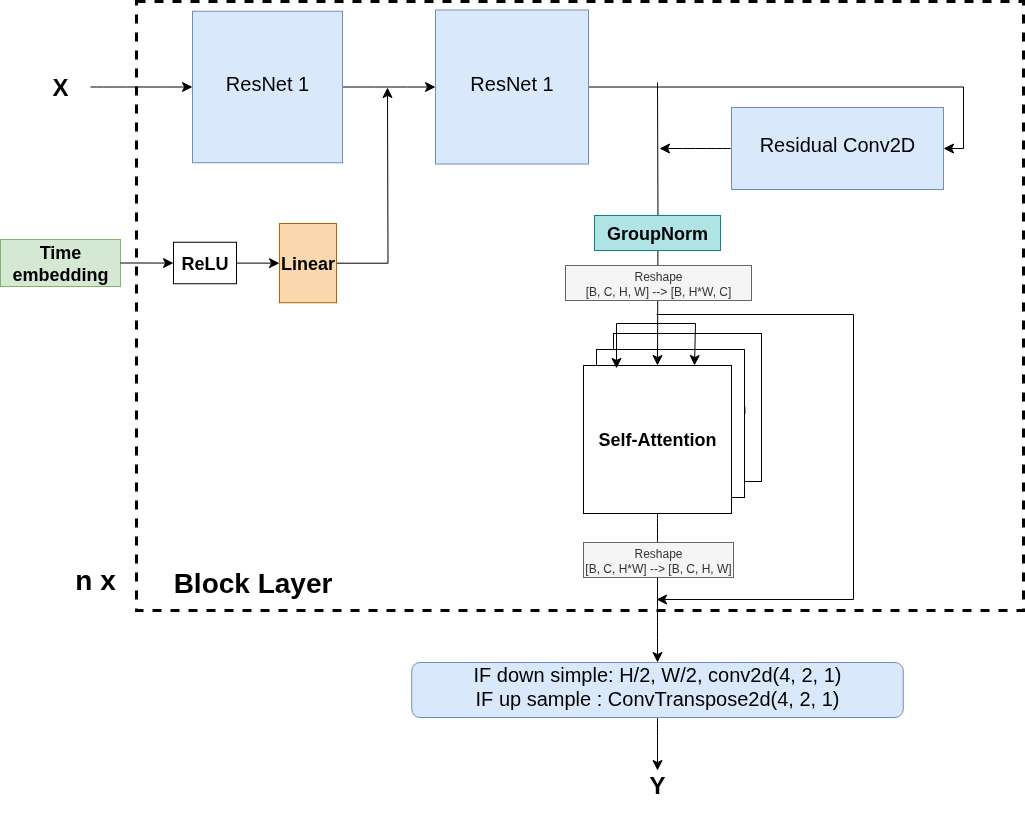
\includegraphics[width=\textwidth]{figures/block_layer.png}
  \caption{Block layer Architecture with ResNet blocks and self-attention layers.}
  \label{fig:unet_architecture}
\end{figure*}

The ResNet block consists of two convolutional layers with Group normalization and SiLU activation, allowing the model to learn residual mappings, and the input is added to a \textbf{positional embedding learnable vector} after the first convolutional layer, whereas the self-attention layer allows the model to focus on relevant features in the input image, improving the quality of the generated images.

The DownEncoder uses strided convolutions to reduce the spatial dimensions, while the UpDecoder uses transposed convolutions to increase them. The Bottleneck uses standard convolutions without striding.


% %%%%%%%%%%%%%%%%%%%%%%%%%%%%%%%%%%%%%%%%%%%%%%%%%%%%%%%%%%%%%%%%%%%%%%%%%%%%%%%%%%%%%%%
\subsubsection{Motivating choices}

\textbf{the choice of activation function:} we choosed SiLU (Sigmoid Linear Unit) as the activation function for the model, which is known to improve the flow of gradients and enhance the model's ability to learn complex features. SiLU has been shown to outperform ReLU in many cases, especially in image-tasks.
in other point of view, image pixels are normalized to the range [-1, 1], and the SiLU activation function is well-suited for this range, as it smoothly transitions between negative and positive values.

\textbf{the choice of normalization:} we used Group Normalization instead of Batch Normalization, to normalize the features within groups, which is more effective in stabilizing training, especially that in our cases where batch size is set to 6 which is small because we hit the GPU's Limit, it is also good for variable batch size while evaluation.

\textbf{the choice of attention mechanism:} as modern architectures often incorporate attention mechanisms, we used self-attention layers to helps the model to capture long-range dependencies and relationships between pixels, which is crucial for generating high-quality images.

the shape of the input of self-attenstion is : $[B, H*W, C_i]$ 
respectively batch, height, weight and out\_channels of a given Block layer. Which makes relationships between pixels more explicit than $[B, C_i, H*W]$.

this mechanism has an impact, as we will see in the cumming sections, that there is a trade-off between an attention block for each block layer and the model's performance, as it increases the number of parameters, requires more data to train, sensible to noise...
% for remark, the impact of not having normalized data in the beginnd was poor sampling with dark images...
we will get a tour over the architecture we have tried in the order time we


\subsubsection{Recaptilative Table:}
\begin{table}[ht]
\centering
\begin{tabular}{|l|c|c|c|c|c|c|c|c|}
\hline
\rotatebox{90}{\textbf{Model Name}} & \rotatebox{90}{\textbf{Params (M)}} & \rotatebox{70}{\textbf{Down Channels}} & \rotatebox{90}{\textbf{down Layers}} & \rotatebox{70}{\textbf{Mid Channels}} & \rotatebox{90}{\textbf{Mid Layers}} & \rotatebox{90}{\textbf{Dropout}} & \rotatebox{90}{\textbf{Attention}} & \rotatebox{90}{\textbf{Time Emb Size}} \\
\hline
mini & 10 & [32,64,128,256] & 2 & [256,256,128] & 2 & 0 & \small{Full} & 128 \\
Simple & 49 & [32,64,128,256,512] & 3 & [512,512,256] & 2 & 0 & \small{Full} & 128 \\
Mega & 74 & [32,64,128,256,512] & 5 & [512,512,256] & 3 & 0.1 & \small{Full} & 128 \\
Giga& 85 & [128,256,256,512] & 5 & [512,512,256] & 5 & 0.1 & \small{Partial} & 128 \\
\hline
\end{tabular}
\caption{Model architecture parameters extracted from training runs.}
\end{table}

NB: $donw channel = up channels$

\subsubsection{Mini U-Net DDPM 10M Architecture:}
this is the model we started with, the idea is to know weither we can reach an acceptable quality of the images, strictely increasing down channels in the DownDecoder, with attention in each block layer.

the model is not capable of generating coherent sampled images, its best performence is reached at the first epochs, and continiousely decreading quality for sampling until generating uncomprehensive noise with almost the same grade of colors.

but the model is still denoising fairly as good as larger models. 
\subsubsection{Simple U-Net DDPM 49M Architecture:}
the second try was to augment the capacity of the model by increasing the number of block layers to 3 and an additional layer of DownEncoder (automatically UpDecoder) to reach 512 channels.

the performence has increased, but the sampling is still poor and not diverse, and reachs the best performance 
in the 3th epochs, an continues with the same assumptoms of previous one.
\subsubsection{Mega U-Net DDPM 74M Architecture:}
here we augmented the capacity of the model by increasing the number of block layers of DownEncoder and UpDecoder to 5, Bottleneck to 3 layers.

the result is a significant improvement in the quality of samples, by epoch 7. but the results sill not that saisfactory, because there is a lake of diversity in hair colors, some darkness themes, lake of sharpness as well as some sort of noisy face patterns.

we notice that epochs between 5 and 9, every epoch has a common samples pattern, such as hair color, face color, sharpness, the model stick to one pattern, similar faces, thus we beleive that attention mechanism has role in this issue as well as the limited size of batch (2)\footnote{The same resource 2x(Nvidia a5000) allows training Mega on 2 batches, while allowing 6 batches for Giga.} .
starting from epoch 10, the samples start to be waters...%TODO
\subsubsection{Giga U-Net DDPM 85M Architecture:}
Here we decided to increase the capacity of the model by increasing the number of channels in the DownEncoder and UpDecoder to 128 and 256 respectively, while keeping the same number of block layers to 5 for both DownEncoder and UpDecoder, and 5 for Bottleneck.

then we decided that a transformer for each block layer may be not a good idea, as it requires too much data to train and more prone to noise, as well as for computaion limited ressource issues, thus in Giga model, we apply the attention layer as follows:

\begin{table}[h!]
\centering
\begin{tabular}{|c|c|c|c|c|c|}
\hline
\textbf{Layer} & \textbf{Pos 1} & \textbf{Pos 2} & \textbf{Pos 3} & \textbf{Pos 4} & \textbf{Pos 5} \\
\hline
Down & False & True & False & True & True \\
Mid  & False & True & False &   -  &  -  \\
Up   & False & True & False & True & False \\
\hline
\end{tabular}
\caption{Attention application across Block layers}
\end{table}
    % down_apply_attention: list = (False, True, False, True, True)
    % mid_apply_attention: list = (False, True, False)
    % up_apply_attention: list = (False, True, False, True, False)
such that the first block layer does not contain an attention layer, the idea is to obtain some meaningful input for the transformer, our best-choice is inspired from GPT, BERT and modern Large languages models that take as input a meaningful semantic vectors from pretrained embedding (word2vec, FastText...), thus we do the same thing for images, as convolution-oriented layers -such ResNet- tend to extract meaningful features from images which can be feed to our transformers.
it also produces cleaner images even in the first epochs, which is not the case with smaller models that contains full transformer.

earliest epochs produce more diversity, and coherent faces which means that

we believe that this significant improvement is not only due to the capacity of the model given the number of parameters, but also to the change of the architecture by omitting some attention layers in the early stages, as well as allowing for bigger batch sizes (at most 6) which lead to a computation stability which can be seen in the train and validation loss plots in the next section.


% In our case, we found that using attention in the first two block layers of the DownEncoder and UpDecoder was sufficient to achieve good results without significantly increasing the model's complexity.


% %%%%%%%%%%%%%%%%%%%%%%%%%%%%%%%%%%%%%%%%%%%%%%%%%%%%%%%%%%%%%%%%%%%%%%%%%%%%%%%%%%%%%%%

% as we progress through epochs, small models tend to overfit very fast, 10M and 49M reaches their best generation respectively 1 and 3 but still very low quality, then they tend to denoise images but very low generation quality, while larger models 74M and 85M tend to perform poorly in earlest epochs, and then  generate better quality images respectivly 7 and %TODO but require more data to train and are more sensitive to noise in later time steps.

%mode colapse, althourht 

%LOSS FUNCTION we choosed to not consider the upsamplinf factor in the MSE $\frac{1}{2\sigma_t^2} \frac{(1 - \sigma_t)^2}{(1 - \hat \sigma_t) \sigma_t}$, our goal is not the maximum likelyhood estimation

% having a 
% having the train and validation loss decreasing to very low valaues doies not mean that our generation quality would improve, in contrast, it leads to somtin g siomilar to data colapse in Hierachical VAEs, where the assumption on the distribution of latent variable is too constraining or when the chaining is too short.

% as we can see with the giga model, as we progress in the training the quality improves, but in the Mega models we reach the best generation performence early between the 6th and 7th epochs, an then the quality is contiinously decreasing.

% what we find surprising is the fact that the models with big capacities

% we also a dded a clap for the loss, because we experienced some huge pics in score based model, as the random variable $\epsilon$ can vary unboundely to not breack the assumption of gaussian noise, thethe solution for that is to clip the values of loss error to a certain range.
\subsection{Training}

Our training technique is based on standard denoising diffusion probabilistic models (DDPM) paper. we trained the model to predict the original noise $\epsilon$ given a noisy image $x_t$ and a time step $t$. The model learns to denoise the image by minimizing the Mean Squared Error (MSE) between the predicted noise and the true noise.

we draw a timestep from a uniform distribution between 0 and T=1000, for $\beta_t$ linearly increasing from $1e-4$ up to $$2e-2$$ a noise $\epsilon$ from normal distribution and a data point from dataset (in batches).

so linear schedule works quit good for these denoising models
\begin{figure*}[h]
  \centering
  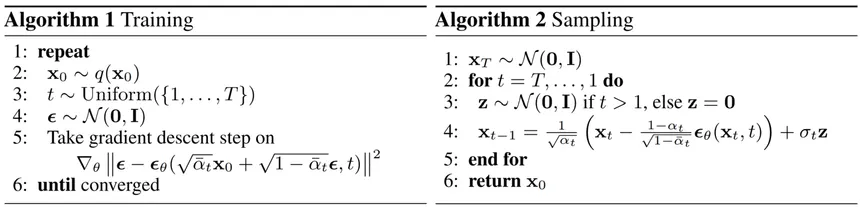
\includegraphics[width=8cm]{figures/training-sampling-algo-ddpm.png}
  \caption{training and sampling algorithm for DDPM.}
  \label{fig:train-sampling-algo-ddpm}
\end{figure*}

\subsubsection{Parameters}
for learning rate, we trained on $1e-4$ for Mini and Simple, and $2e-4$ for Giga and Mega models.

\subsubsection{Training Procedure}

\subsubsection{Optimizer}
We used the AdamW optimizer, which is an extension of the Adam optimizer with weight decay. AdamW helps to prevent overfitting by adding a weight decay term to the loss function, which dampens oscillations and large gradients.

the desicion to use AdamW was based on its effectiveness in training deep learning models, especially in the context of image tasks. It combines the benefits of adaptive learning rates and weight decay.

we kept the default parameters for AdamW, which are:
\begin{table}[h]
    \centering
    \begin{tabular}{|c|c|c|c|c|}
        \hline
        $\beta_1$ & $\beta_2$ & $\epsilon$ & weight decay & learning rate \\
        \hline
        0.9 & 0.999 & 1e-8 & 1e-4 & 1e-4 \\
        \hline
    \end{tabular}
    \caption{Optimizer Parameters}
    \label{tab:optimizer_params}
\end{table}

\subsubsection{Loss Function}
the loss function used for training the models is Mean Squared Error. It measures the dissimilarity between the predicted noise and the true noise.
The Mean Squared Error loss is defined as:
\[
\mathcal{L} = \mathbb{E}_{x \sim p(x), t \sim \mathcal{U}, \epsilon \sim \mathcal{N} } ||(\epsilon - \epsilon_\theta (x_t, t))||^2
\]
we choosed to not consider the upsampling factor in the MSE $\frac{1}{2\sigma_t^2} \frac{(1 - \sigma_t)^2}{(1 - \hat \sigma_t) \sigma_t}$, our goal is not the maximum likelyhood estimation but a better samples.



\begin{figure*}[ht]
    \centering
    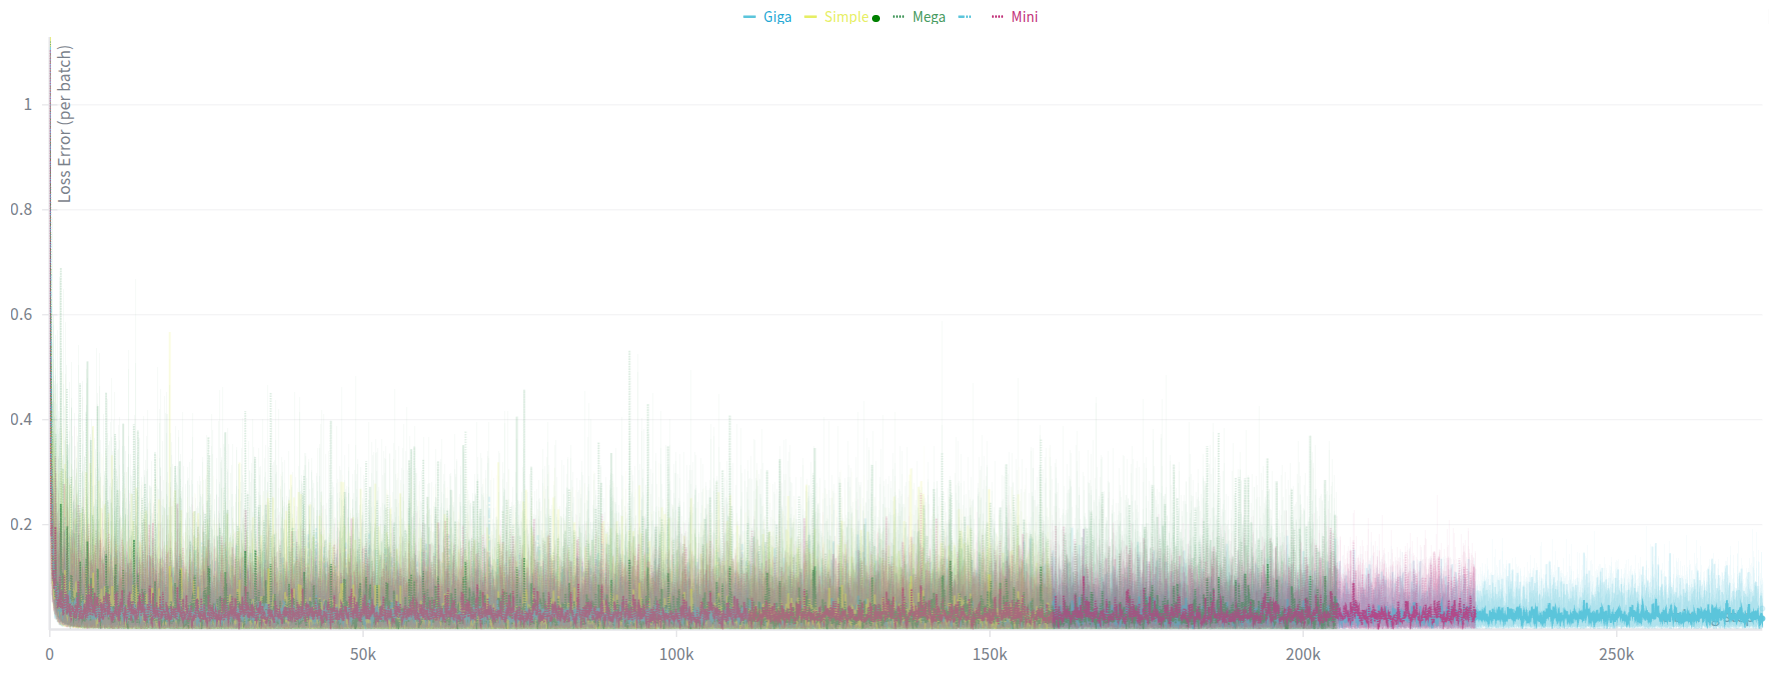
\includegraphics[width=\textwidth]{figures/train----Screenshot from 2025-08-13 19-55-18.png}
    \caption{Evolution of Train Loss per step for each model.}
    \label{fig:train-losses}
\end{figure*}

\begin{figure*}[ht]
    \centering
    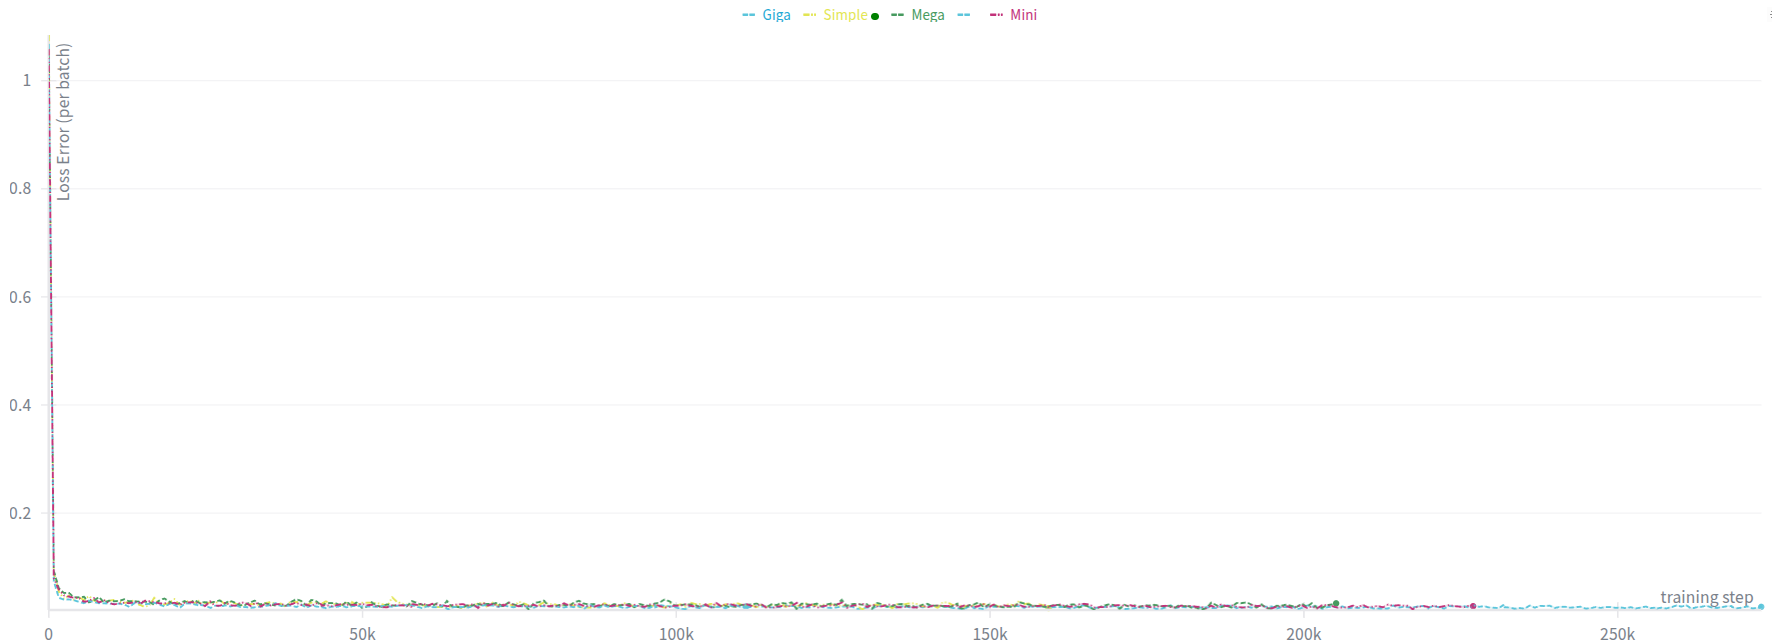
\includegraphics[width=\textwidth]{figures/validation--Screenshot from 2025-08-13 19-56-31.png}
    \caption{Evolution of Validation Loss per step for each model.}
    \label{fig:val-losses}
\end{figure*}

\section{Results}

\section{Discussion} %and future improvements


\subsection{The importance of }


\subsection{The importance of }


\subsection{The importance of cropping images}

\subsection{About possible improvements}


% ==============================================================================
\subsection{The deceiving performance of Score-based Energy model}

we followed the preconditioning and sampling strategy of the paper \cite{karras2022elucidating} to train a score-based energy model, which is a generative model that learns to approximate the score function of the data distribution. The model is trained to predict the score function at different noise levels, and it can generate samples by sampling from the learned distribution.

we obsered very poor of ED, such that we observed some huge fletuations in the train losses that varies from 0.01 to more than 4000 , which indicates unstability 



% ==============================================================================
\newpage
\section{References}

\bibliographystyle{IEEEtran}
\bibliography{bibliography}

\end{document}